\section{Demystifying Side Effects}

Modern kernel exploit development often involves deriving new (and often stronger) exploit primitives from unintended memory operations caused by a bug. These operations rarely appear in isolation: one bug-triggering path may perform several writes, frees, or pointer dereferences. In this paper, we call such unintended memory operations \emph{effects}. Once an exploit strategy selects one effect as the desired primitive, the remaining effects on that same path become \emph{side effects}. In many cases, side effects can prevent an exploit from working altogether (e.g., causing crashes), making them a critical obstacle to successful exploitation.

In this section, we use a motivating example to illustrate the intricate relationship between primitives and side effects.

% We then propose two generic strategies to mitigate side effects and facilitate exploitation of the vulnerability. Finally, we discuss the limitations of existing state-of-the-art primitive discovery frameworks in handling side effects.


% \zhiyun{consider citing some numbers from syzscope to highlight the number of primitives per bug.}
\subsection{Motivating Example}


\begin{figure}[htbp]
    \centering
    \begin{minipage}[t]{\linewidth}
        \begin{lstlisting}[language=C]
SYSCALL_DEFINE0(F)
{
    free(obj);                    <@ \circled{1} @> Unexpected Free
}

SYSCALL_DEFINE1(A, long, arg1)
{
    obj->f1 = 0xdeadbeef;         <@ \circled{2} @> UAF Write
    if (arg1)                     <@ \circled{4} @>
        obj->p1->f2 = 0xdeadbeef; <@ \circled{5} @> AAW
    obj->func();                  <@ \circled{6} @> CFH
}

SYSCALL_DEFINE0(B)
{
    obj->p2->f3 = 0xdeadbeef;     <@ \circled{3} @> AAW
    if (obj->field)               <@ \circled{7} @>
        obj->func();              <@ \circled{8} @> CFH
}
\end{lstlisting}
    \end{minipage}
    
    \caption{Code for the motivating example}
    \label{fig:motivating_code}
    \vspace{-1 pt}
\end{figure}


\vspace{-0.3cm}
\begin{figure}[htbp]
  \centering \def\svgwidth{\columnwidth} 
  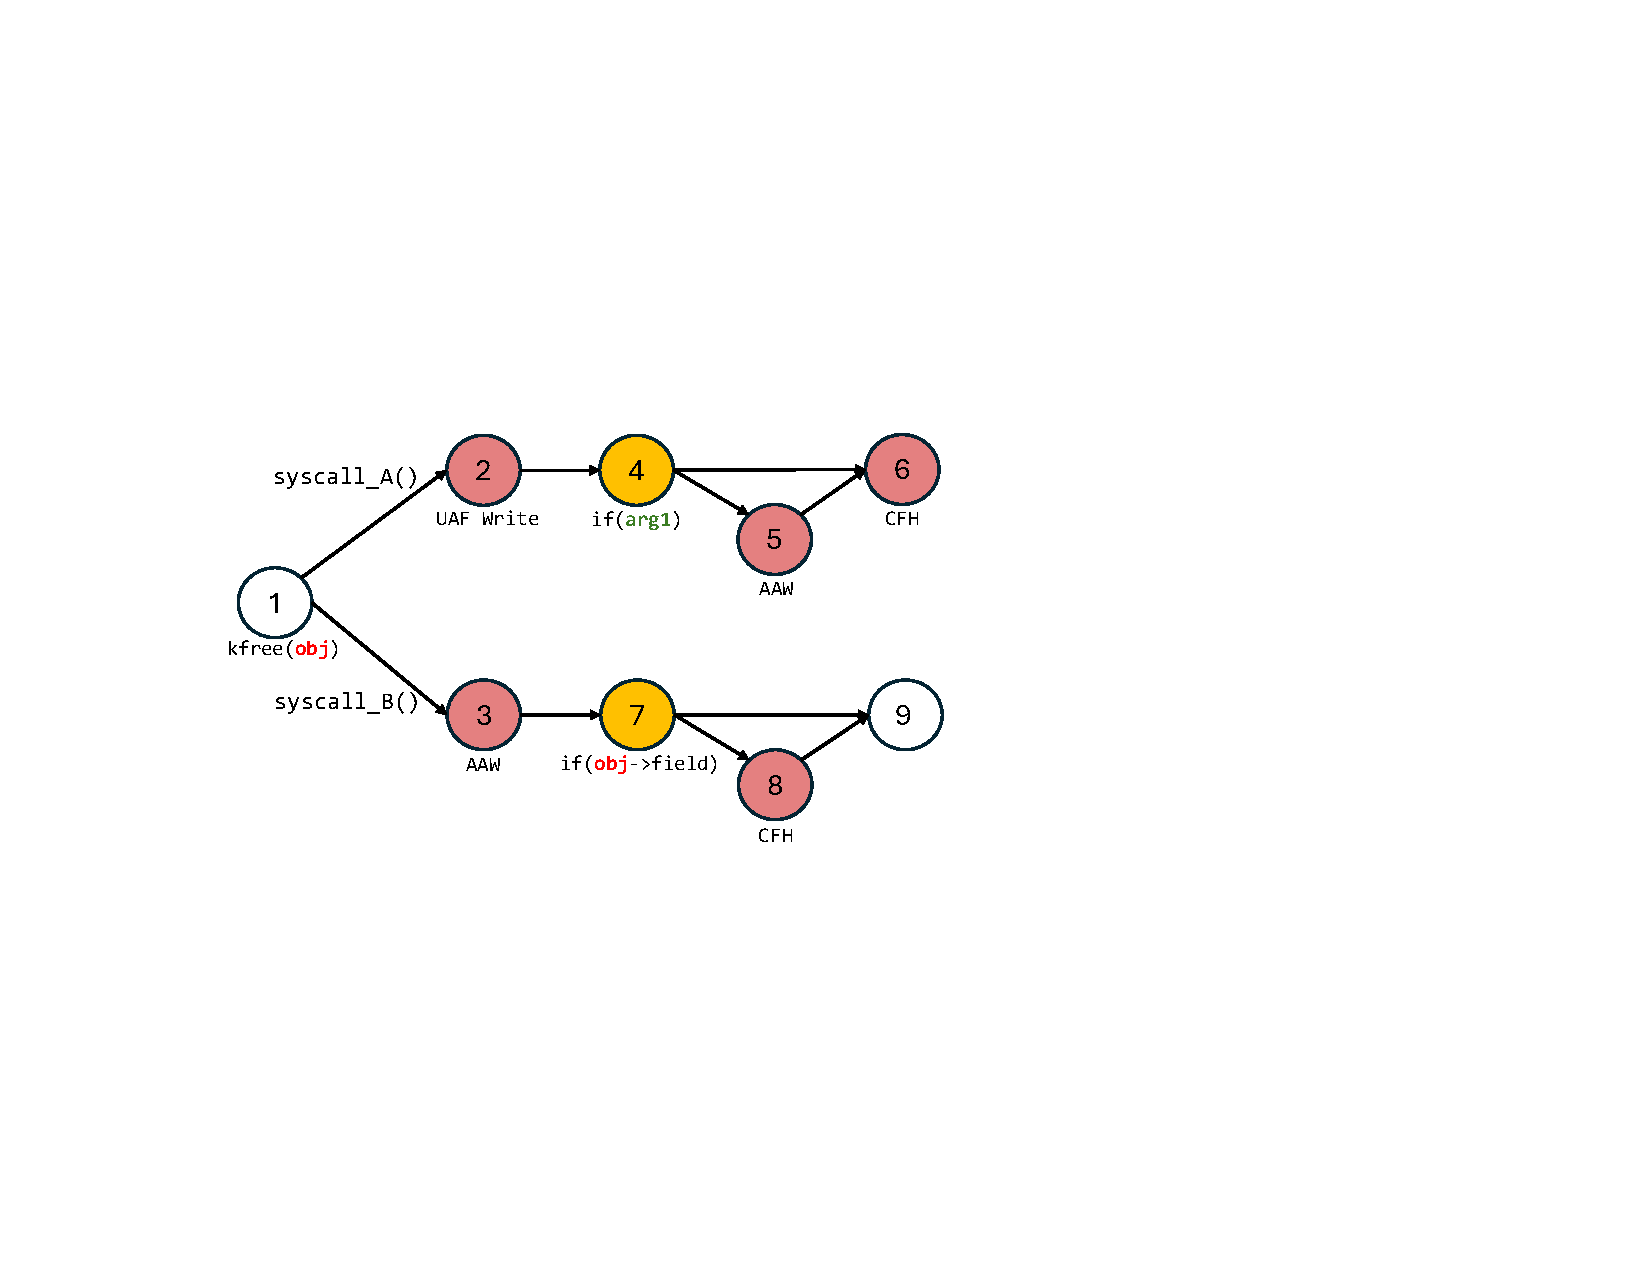
\includegraphics[width=\linewidth, trim=80 200 200 205, clip]{./figures/motivating.pdf}
  \vspace{-0.5cm}
  \caption{\label{fig:motivating}The motivating example kernel vulnerability}
\end{figure}
% \zhiyun{is this a control flow graph? need to explain}


The motivating example is a UAF bug simplified from a real kernel bug.
The corresponding kernel code can be found in Figure~\ref{fig:motivating_code}, and a control flow graph annotated with potential primitives is depicted in Figure~\ref{fig:motivating}. In this bug, \textcolor{red}{\texttt{obj}} is freed, illustrated at \circled{1} in Figure~\ref{fig:motivating}, but there are two potential syscall invocations (\texttt{syscall\_A()} and \texttt{syscall\_B()}) that can still access a dangling pointer, leading to a use-after-free bug.

% \zhiyun{The description of the example is incomplete. We need to explain there are multiple primitives associated with different syscalls. Within each syscall, there are also multiple primitives --- reachable via different paths. Then we can explain why there may be side effects, if we want to choose, say the CFH primitive for exploitation. In fact, I think we will need some pseudocode to illustrate this. I drafted the beginning of a new paragraph below.}

As we can see from the simplified syscall implementations in Figure~\ref{fig:motivating_code}, an attacker can invoke \texttt{syscall\_A()} to potentially trigger 3 primitives: UAF Write, Arbitrary Address Write (AAW) and Control Flow Hijacking (CFH). On the other hand, invoking \texttt{syscall\_B()} will potentially trigger 2 primitives: AAW and CFH.

To influence the behaviors of the vulnerability and steer the kernel into different execution paths, the attacker can choose the bug-triggering syscall (i.e., \texttt{syscall\_A()}, \texttt{syscall\_B()}, or modify syscall arguments such as \textcolor{DarkGreen}{\texttt{arg1}} to alter the vulnerability context. Furthermore, the attacker can leverage heap spray to manipulate the memory pointed to by the dangling \textcolor{red}{\texttt{obj}} pointer, thereby influencing the execution paths in \texttt{syscall\_B()}.

Suppose the attacker’s goal is to hijack kernel control flow using a CFH primitive. One option is to invoke \texttt{syscall\_A()} and spray attacker-controlled data to reclaim the freed memory. However, this path deterministically triggers UAF Write at \circled{2}, and may also trigger an AAW at \circled{5}. 
%Here, \emph{AAW side effect} denotes an undesirable effect in which a pointer corrupted by sprayed data is dereferenced (the attacker may not know a valid address to place in that pointer field).
Both can crash the kernel. UAF Write may corrupt critical fields of the reclaimed object, causing later failure when that object is used. AAW is more severe, because dereferencing a corrupted pointer (e.g., \texttt{obj->p1}) can immediately fault if it points to an invalid address.

% \zc{Only an intended AAW by the attacker is called AAW; "AAW" side effect should be called dereferencing invalid write pointer, as the attacker has no intention to specify the address}\juefei{Changed}
%In this scenario, AAW \circled{5} is considered a primitive, and CFH \circled{6} is considered a side effect, as the attacker only wants to use AAW to corrupt the global variable and he does not want to alter the kernel control flow.
% Along these potential execution paths, there are effects such as UAF Write, Arbitrary Address Write (AAW), Control Flow Hijack (CFH).

\subsection{Effects, Primitives, and Side Effects} \label{chap:eps}

We begin by defining key terms that set the foundation for the rest of the paper.

\textbf{Effects} refer to any unintended memory operations directly or indirectly caused by the vulnerability.

\textbf{Primitives} are a subset of effects, denoting the specific effects that attackers choose to carry out an exploit. In the motivating example, if the attacker selects the CFH effect, e.g., to conduct return-oriented programming, we consider the CFH effect a primitive.

\textbf{Side effects} are defined as the remaining effects that occur together with the primitive, but are not chosen for exploit construction.

We make three key observations about these definitions.

\noindent\textbf{1. Primitives Are Chosen}: Whether an effect is considered a primitive depends on the attacker's strategy. For example, although CFH is often seen as powerful (e.g., for ROP), if the attacker chooses to use UAF Write instead (to corrupt heap objects), the CFH would become a side effect, which can lead to crashes if we do not overwrite it with a legitimate kernel function address.

\noindent\textbf{2. We Model One Selected Primitive at a Time}: 
Real exploits may combine multiple effects across repeated triggers or exploit stages. For tractable per-path accounting, SyzPass models one selected primitive site for one exploit strategy and treats the remaining effects on that same path as side effects. SyzPass initially treats each effect site as a possible selected-primitive hypothesis; primitive-specific preservation rules later decide whether that hypothesis remains useful on the analyzed path.

\noindent\textbf{3. Some Side Effects Are More Lethal}: 
Not all side effects are equally harmful. Side effects involving pointer dereferences are especially dangerous because they can fail immediately when the corrupted pointer field is filled with an invalid value (e.g., 0x0 from zero-initialized spray objects). For example, CFH and AAW are typically riskier than UAF Write: if the reclaimed object is zero-initialized and a pointer field is dereferenced without validation, the kernel will crash.

%\zhiyun{need to define purified primitives or clean primitives. I personally prefer clean because purified assumes it requires work to be clean (but a primitive may naturally be clean and does not require purification).}

%\zhiyun{The definitions here are much clearer (and more reasonable) than the ones in the opening paragraph. We should improve the opening paragraph to match the actual definition.}

%As a result, in this paper, we \textbf{do not} determine primitives based on the behaviors of effects. Instead, we leave the freedom of choosing the exploit strategy to the exploit developer and treat all effects as potential primitives equally. Thus, for each of them, we try to find strategies to solve other effects for it. In addition, we prioritize solving side effects involving pointer dereferences.

In this paper, we \textbf{do not} determine primitives from behaviors of effects. Instead, we leave exploit-strategy selection to the developer and treat all effects as potential primitives. For each potential primitive, we then seek mitigation strategies for the remaining effects (i.e., side effects). We further prioritize mitigating side effects that involve pointer dereferences.


% For each potential primitive provided by the vulnerability, we assume the attacker chooses it as the primitive for the exploit, then treat all other unintended memory operations as side effects to be minimized


% Whether an effect is useful is largely subjective, depending on the attacker's strategic preferences. In our motivating example, all three effects might be chosen as the primitive for exploit development. UAF Write can be used to corrupt critical fields of other heap objects, AAW can be used for corrupting global variables, and CFH can be used to conduct ROP. However, regardless of which effect is chosen as the primitive, others effects becomes useless and then become side effects due to their contrary to the chosen exploit strategy. 


% In the motivating example, both AAW and CFH are generally viewed as promising effects. An experienced attacker may either choose AAW as the primitive and tamper critical global variable or choose CFH as the primitive and conduct ROP to achieve privilege escalation. However, regardless of which primitive is chosen, others effects becomes side effects.

% And side effects caused by AAW and CFH are especially fatal since involved pointer dereference and the risk of kernel crash. From the attacker's perspective, side effect \textbf{avoidance} and \textbf{neutralization} are two generic approaches dealing them.


% Furthermore, SyzScope does not associate the primitive with execution trajectory after triggering it (i.e., \circled{5}$\rightarrow$\circled{6}, \circled{3}$\rightarrow$\circled{7}$\rightarrow$\circled{9}, \circled{3}$\rightarrow$\circled{7}$\rightarrow$\circled{8}$\rightarrow$\circled{9}), completely missing effects after behind each primitive. Consequently, SyzScope's primitive reports provide very limited help for attackers.

% its report often lacks enough practicality to guide the attacker to develop an exploit. First, for each primitive, SyzScope only reports its exist and the first path SyzScope found towards it. For instance, for the AAW primitive, it may only reports \circled{1}$\rightarrow$\circled{3} 

% First, for each primitive, SyzScope only reports the first path to reach it, without alternative paths to reach it, and does not reason for paths after it. For instance, for the AAW primitive, it only reports \circled{1}$\rightarrow$\circled{3} or \circled{1}$\rightarrow$\circled{2}$\rightarrow$\circled{4}$\rightarrow$\circled{5} (based on which one is firstly executed) not both of them. And SyzScope does not reason whether the path can safely reach the end of syscall without triggering additional side effects. 

% First, for each primitive, SyzScope only reports the first path it discovers reaching it, failing to analyze other alternative paths with fewer side effects in a holistic way. For instance, for the AAW primitive. It only reports \circled{1}$\rightarrow$\circled{3}

% Second, SyzScope implicitly assumes the attacker can forge arbitrary level of kernel pointers to exploit the vulnerability, overly simplify the modeling of side effects. However, in practice, the attacker has limited ability to forge the kernel pointers, and report that requires the attacker to forge such pointer become meaningless


% Introduce side effect here


% How SyzScope would do that and How GREBE would do that

% In fact, these represent everything the attacker can control in the scenario of exploit development. Therefore, an effective side effects mitigation strategy must be based on either (1) adjusting the syscall or (2) manipulating the sprayed memory.

% It is a UAF bug, where the object is freed at \circled{1}, but can be used later.

% in the implementation of the \texttt{AF\_PACKET} socket within the \texttt{net} subsystem. The affected object is the \texttt{sk\_buff}, which represents a packet in the Linux kernel.

% The vulnerability arises from the mishandling of packets received through the \texttt{AF\_PACKET} socket. This error causes the kernel to free an \texttt{sk\_buff} object while leaving it in the doubly linked list associated with the socket. Therefore, as shown in Figure~\ref{fig:motivating}, an attacker can trigger the vulnerability in different ways by using various syscalls to interact with the socket.
% % To influence the behavior of the vulnerability, the attacker can change the syscall they execute to achieve that. Meanwhile, the behavior of the vulnerability is also influenced by syscall arguments, such as \textcolor{DarkGreen}{\texttt{flags}} and \textcolor{DarkGreen}{\texttt{len}}. Additionally, an attacker can also leverage heap spray to manipulate the memory pointed by the dangling \textcolor{red}{\texttt{skb}} pointer, and thus influence the behavior of the vulnerability.

% To influence the behavior of the vulnerability, the attacker can choose a different syscall. Meanwhile, the behavior of the vulnerability is also influenced by syscall arguments, such as kernel variables \textcolor{DarkGreen}{\texttt{flags}} and \textcolor{DarkGreen}{\texttt{len}}, which are controled by the syscall argument. Additionally, an attacker can leverage heap spray to manipulate the memory pointed to by the dangling \textcolor{red}{\texttt{skb}} pointer, thereby influencing the behavior of the vulnerability. 

% In fact, these represent everything the attacker can control in the scenario of exploit development. Therefore, from the attacker's perspective, effective side effects mitigation strategies should focus on two primary approaches: (1) adjusting the syscall, and (2) manipulating the sprayed memory.





% 1. Side effect avoidance via Syscall Manipulation

% 2. Side effect avoidance via Sprayed Memory

% 3. Side effect neutralization.
